% ============================= SITE =============================
\section{External Validation on SITE (ICCV 2025)}
\label{sec:site}

The VSR findings could be benchmark-specific. Before any evaluation, we
preregistered an external-validation protocol on SITE~\cite{wang2025site}
(config hash \texttt{28f4cc09887477af}; frozen example IDs in
\texttt{results/site/site\_protocol.json}; evaluation-only, no SITE training).
The decision rule: if the official spatial-relationship category is broadly
weak, run the VSR-trained LoRA; if \emph{only} the orientation-vocabulary subset
is weak, narrow the claim to object/direction orientation; if neither, the VSR
finding is benchmark-specific.

\subsection{Results}
We evaluated Qwen2-VL-7B-Instruct zero-shot on all 2{,}591 image examples
(Table~\ref{tab:site}, Fig.~\ref{fig:site}).

\begin{table}[t]
\centering
\footnotesize
\setlength{\tabcolsep}{2.3pt}
\begin{threeparttable}
\caption{\textbf{SITE external validation, 7B zero-shot (images)}. Raw
accuracy and official chance-adjusted accuracy (CAA) with Wilson 95\% CIs.
Secondary subset numbers recomputed from the committed prediction CSV and
consistent with the frozen protocol ($n{=}2{,}024$ image examples).}
\label{tab:site}
\begin{tabular}{lccc}
\toprule
Subset & $n$ & Raw acc.\ (\%) & CAA (\%) \\
\midrule
All images & 2{,}591 & 54.2 $[52.3, 56.1]$ & 31.1 \\
Primary: spat.-rel.\ reasoning\tnote{a} & 993 & \textbf{75.1} $[72.3, 77.7]$ & \textbf{59.2} \\
Secondary: orient.\ keywords\tnote{b} & 2{,}024 & 48.3 $[46.2, 50.5]$ & 24.0 \\
\midrule
single-image & 1{,}368 & 61.3 & 37.4 \\
multi-image & 1{,}223 & 46.4 & 24.9 \\
\bottomrule
\end{tabular}
\begin{tablenotes}\footnotesize
\item[a] Official category; the preregistered headline subset.
\item[b] Non-official keyword-derived heuristic subset; supporting analysis
only (exact keyword rule in App.~E).
\end{tablenotes}
\end{threeparttable}
\end{table}

\textbf{(1) Spatial-relationship reasoning is not broadly weak.} The official
category reaches 75.1\% raw / 59.2\% CAA --- comparable to or above published
open-source results on this category (e.g., Qwen2.5-VL-7B at 51.5\% CAA on the
SITE leaderboard). VSR statements embedded in SITE score 85.9\% / 71.8\%, and
synthetic sources (CLEVR 92.6\%, IconQA 91.5\%) are near-saturated. A
representative, in-the-wild model is \emph{good} at spatial relations broadly.

\textbf{(2) Orientation-vocabulary questions collapse.} The secondary subset
drops to 48.3\% raw / 24.0\% CAA --- a 26.8-point raw / 35.2-point CAA gap to the
primary subset, driven by the same vocabulary as VSR's orientation family
(facing, direction, view, rotation, left/right, parallel/perpendicular). The
effect is consistent across sources: orientation-heavy corpora (exoego4d 36.4\%,
egoexo4d 34.7\%, SAT 46.4\%, MMIU 34.2\%) sit far below the source average,
while the same model saturates relation-heavy sources. The 392-px resolution cap
(constant protocol parameter) cannot explain the gap: high-resolution
multi-image sources such as CLEVR (92.6\%) do fine, and the deficit concentrates
precisely in orientation-vocabulary questions.

\begin{figure*}[t]
\centering
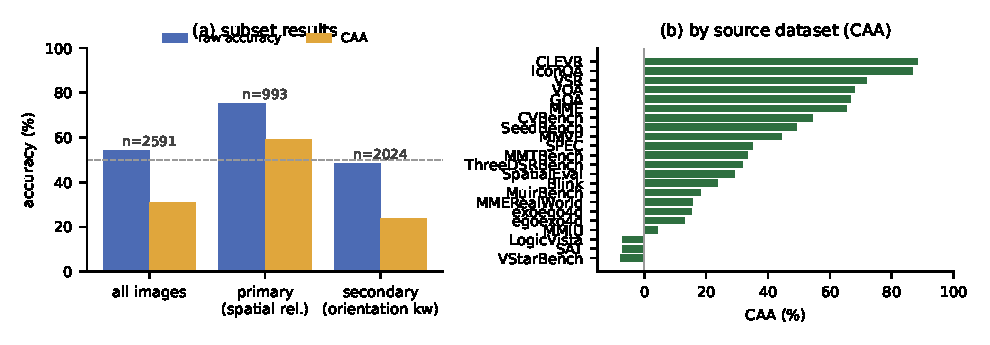
\includegraphics[width=\textwidth]{fig/site_validation.pdf}
\caption{\textbf{SITE external validation (7B zero-shot, images).}
(a) Raw accuracy and CAA by subset: the official spatial-relationship category
is comparatively strong while the orientation-keyword subset collapses.
(b) CAA by source dataset (n$\geq$30): orientation-heavy corpora (SAT, MMIU,
exoego4d, egoexo4d, LogicVista) are at or below zero CAA, while
relation-heavy sources saturate.}
\label{fig:site}
\end{figure*}

\textbf{Decision-rule outcome (branch 2, preregistered):} the VSR orientation
finding \emph{generalizes to SITE}, specifically for object/direction
orientation --- not for spatial-relationship reasoning broadly. The paper's
claim is accordingly narrowed: \emph{VLMs show a persistent,
benchmark-independent weakness in object-intrinsic orientation (facing/
direction), while general spatial-relationship reasoning is comparatively
strong}.

\textbf{Reproducibility discrepancy note.} The run-time metrics JSON
(\texttt{zeroshot\_image\_metrics.json}) records the secondary subset with
$n{=}1{,}824$ (47.3\% raw / 22.6\% CAA), while the committed prediction CSV ---
consistent with the frozen protocol's image IDs ($n{=}2{,}024$) --- gives the
numbers above; all other numbers (all/primary/modality/sources) are bit-identical
between the two artifacts. We report the CSV+protocol-consistent values and
document the discrepancy in App.~G. Both values support the same
conclusion.
